%% KO_template.tex
%% V2015
%% by Jan Dvořák
%% based on
%% bare_conf.tex
%% V1.3
%% 2007/01/11
%% by Michael Shell

%%*************************************************************************
%% Legal Notice:
%% This code is offered as-is without any warranty either expressed or
%% implied; without even the implied warranty of MERCHANTABILITY or
%% FITNESS FOR A PARTICULAR PURPOSE! 
%% User assumes all risk.
%% In no event shall IEEE or any contributor to this code be liable for
%% any damages or losses, including, but not limited to, incidental,
%% consequential, or any other damages, resulting from the use or misuse
%% of any information contained here.
%%
%% All comments are the opinions of their respective authors and are not
%% necessarily endorsed by the IEEE.
%%
%% This work is distributed under the LaTeX Project Public License (LPPL)
%% ( http://www.latex-project.org/ ) version 1.3, and may be freely used,
%% distributed and modified. A copy of the LPPL, version 1.3, is included
%% in the base LaTeX documentation of all distributions of LaTeX released
%% 2003/12/01 or later.
%% Retain all contribution notices and credits.
%% ** Modified files should be clearly indicated as such, including  **
%% ** renaming them and changing author support contact information. **
%%
%% File list of work: IEEEtran.cls, IEEEtran_HOWTO.pdf, bare_adv.tex,
%%                    bare_conf.tex, bare_jrnl.tex, bare_jrnl_compsoc.tex
%%*************************************************************************


%%!!!!!!!!!!!!!!!!!!!!!!!!!!!!!!!!!!!!!!!!!!!!!!!!!!!!!!!!!!!!!!!!!!!!!!!!!
%%
%% Remove all itemize environments and replace them by your own text! 
%%
%%!!!!!!!!!!!!!!!!!!!!!!!!!!!!!!!!!!!!!!!!!!!!!!!!!!!!!!!!!!!!!!!!!!!!!!!!!



\documentclass[onecolumn, conference]{IEEEtran}

% Uncomment for semester project in czech language
%\usepackage[czech]{babel}

%Uncomment for setting up your encoding (according to *.tex encoding you use)
%\usepackage[latin2]{inputenc} %for windows users
\usepackage[utf8]{inputenc} %for linux users

\usepackage{graphicx}
\usepackage{hyperref}


\newcommand{\range}[2][0]{Range: #1 to #2 page} 
\newcommand{\conciseItem}{\itemsep1pt \parskip0pt \parsep0pt}

\begin{document}
%
% paper title
% can use linebreaks \\ within to get better formatting as desired
\title{Comparison of Matrix Multiplication}


% author names and affiliationsb
% use a multiple column layout for up to three different
% affiliations
\author{\IEEEauthorblockN{Petr Kucera}
\IEEEauthorblockA{
Monday 18h\\
\textit{Open Informatics, Computer Engineering}\\
\textit{kucerp28@fel.cvut.cz}}
}

% make the title area
\maketitle
\section{Methodology}
\subsection{Warm-up}
\begin{itemize}
	\conciseItem
	\item I conducted the warm-up measurement using the methodology outlined in the assignment. Following that, I ran a benchmark test involving 30 warm-up iterations, 100 measured interactions, and 10 forks.
\end{itemize}
\subsection{Measurements}
\begin{itemize}
	\conciseItem
	\item Brief description of how the time performance is measured.
\end{itemize}
\subsection{Comparison}
\begin{itemize}
	\conciseItem
	\item Brief description of how the implementations are compared.
\end{itemize}
\section{Machine specification}
\begin{itemize}
	\conciseItem
	\item CPU, memory, OS, etc.
	\item JVM parameters if used.
\end{itemize}
\section{Results}
\subsection{Warm-up}
\begin{itemize}
	\conciseItem
	\item The initial results were unsatisfactory. The error was likely due to running the program in WSL with insufficient prioritization and performance, thus being influenced by other factors. Nevertheless, I initiated the benchmarking program with 50 warm-up iterations and 50 forks, monitoring the terminal output to observe how the data changes.
	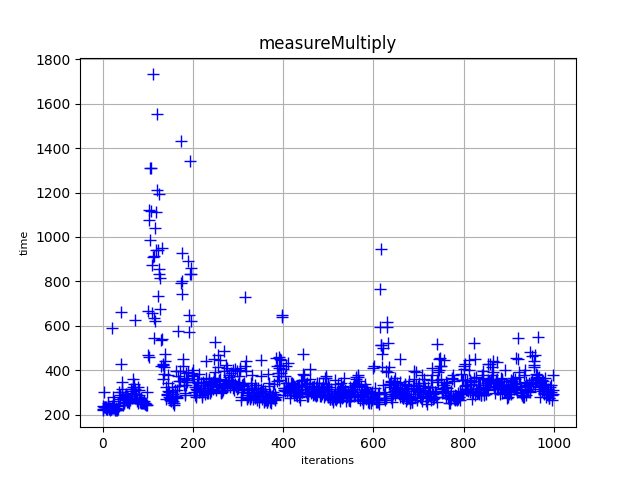
\includegraphics[width=0.3\textwidth]{warmup_measureMultiply.png}
	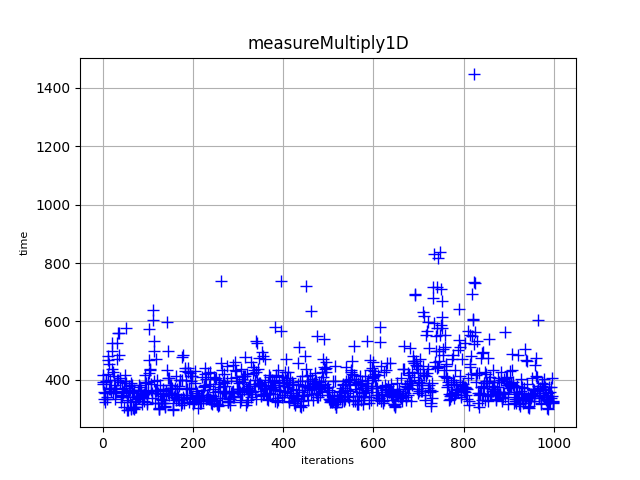
\includegraphics[width=0.3\textwidth]{warmup_measureMultiply1D.png}
	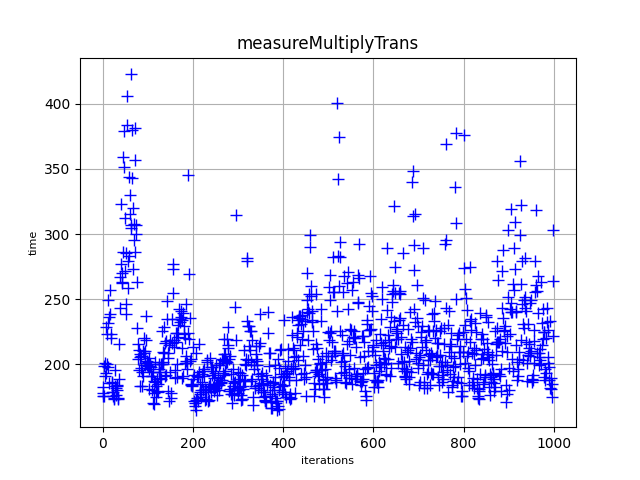
\includegraphics[width=0.3\textwidth]{warmup_measureMultiplyTrans.png}
	\item After analyzing the data, I discovered that the program consistently starts very quickly, and the warm-up only affects the initial launch. Subsequent errors are related to other programs running concurrently with the benchmark. The data can be reviewed in the project repository: \url{https://github.com/petrkucerak/ESW/tree/main/hw/hw04/assets}.
\end{itemize}
\subsection{Measurements}
\begin{itemize}
	\conciseItem
	\item Results of the time measurements including a graph with displayed confidence intervals and a table.
\end{itemize}
\subsection{Comparison}
\begin{itemize}
	\conciseItem
	\item Results of the comparison of the implementations.
\end{itemize}


\section{Conclusion}
\begin{itemize}
	\conciseItem
	\item Summary of the results with a discussion
\end{itemize}

\end{document}
